\documentclass[fontset=none]{article}
\usepackage[]{ctex}
\usepackage[a4paper, total={6in, 8in}]{geometry}
\usepackage{float}
\usepackage{underscore}
\title{LSM-KV 项目报告}
\author{王雨杭 522021910183}
\date{2024年 5月 22日}

\usepackage{natbib}
\usepackage{graphicx}
\usepackage{enumitem}
\bibliographystyle{plain}

\begin{document}

\maketitle

\section{背景介绍}
LSM-KV 是一个基于日志结构合并树(Log-Structured Merge-tree,简称 LSM tree)的键值存储系统。LSM tree 是一种磁盘存储数据结构,用于处理大量随机写入的情况。它通过将随机写入转化为顺序写入,从而提高写入性能。
LSM-KV 项目的主要目标是实现一个高性能、可扩展的键值存储系统。它主要用于处理大数据应用,如搜索引擎、数据库和文件系统等,这些应用需要处理大量的数据写入和查询。同时,LSM tree也是RocksDB、LevelDB、HBase以及Prometheus等知名开源项目底层的存储引擎的数据结构,具有很高的学术和工业应用价值。

LSM-KV 的主要特点包括:
1. 高性能:通过使用 LSM tree,LSM-KV 可以提供高性能的数据写入和查询。
2. 可扩展性:LSM-KV 设计为可以在多台机器上分布式运行,从而处理大规模的数据。
3. 持久性:LSM-KV 使用磁盘存储数据,因此即使在系统崩溃后,数据也不会丢失。
4. 支持多种数据类型:LSM-KV 不仅可以存储简单的键值对,还可以存储更复杂的数据类型,如列表、集合和哈希表等。
这些特点使 LSM-KV 成为处理大数据应用的理想选择。

对比B+树等持久化数据结构,LSM树具备一些专门为记录日志等磁盘写入密集型应用优化的特性,它的主要优势有写入效率高(LSM tree通过缓存写入操作并批量进行,可以显著减少磁盘I/O操作,从而提高写入效率)、高效的磁盘空间利用(LSM tree通过合并和压缩操作,可以有效地利用磁盘空间,减少数据冗余)、高并发性能好等,但在读取效率上存在一定的劣势。

在本项目之中,实现了基本的键值类型为{int, string} 的键值存储LSM树,支持GET、PUT、DELETE和SCAN操作, 并实现了键值分离存储、支持GC、持久性和缓存、修改布隆过滤器大小等配置的特性。

% 这是一个对图片的引用, 图~\ref{fig:universe},以及参考文献~\cite{adams1995hitchhiker}。

% \begin{figure}[h!]
%   \centering
%   \includegraphics[width=0.5\textwidth]{universe}
%   \caption{The Universe}
%   \label{fig:universe}
% \end{figure}

\section{测试}
此部分主要是展现你实现的项目的测试,主要分为下面几个子部分。测试部分应当是文字加上测试数据的图片展示。

我的测试实现如下:在使用cache和Bloom Filter,使用Cache不使用Bloom Filter,两者都不使用三种情况下以及都使用,改变BloomFilter大小为1024 * i(i从1到15变化)字节几种情况,数据(value)大小分别为[10, 100, 1000, 10000]字节,开始GET,POST,DEL, SCAN前已有分别为[1000, 3000, 5000]组随机数据的情况下进行测试,每次测试随机GET 10000次取平均,PUT 1000次取平均, DEL 1000次取平均, SCAN 100次(范围随机)取平均测量耗时和吞吐量。
\subsection{性能测试}


\subsubsection{预期结果}
基于LSM tree的特性,应该表现出:
1. GET请求较慢,在使用缓存的情况下,会稍快
2. PUT和DEL请求较快,且由于DEL请求最坏只需要PUT一个小字符串,DEL应该比PUT更快
3. SCAN请求非常慢,因为要遍历每一层,与GET,PUT,DEL可能有数量级差距
4. 在触发合并时,PUT请求会显著变慢
\subsubsection{常规分析}

\begin{enumerate}
    \item 包括Get、Put、Delete、Scan操作的延迟,你需要测出不同数据大小时的操作延迟,为了测试的合理性,你应当对每个数据大小测量然后计算出平均延迟
    \begin{table}[H]
    \centering
    \begin{tabular}{|c|c|c|c|c|c|}
    \hline
    value\_size & prebuilt_data_num & Get & Put & Del & Scan \\
    \hline
    10 & 1000 & 1 & 4 & 0 & 24 \\
    100 & 1000 & 2 & 4 & 0 & 26 \\
    1000 & 1000 & 9 & 7 & 0 & 23 \\
    10000 & 1000 & 99 & 57 & 0 & 39 \\
    10 & 3000 & 5 & 11 & 0 & 868 \\
    100 & 3000 & 4 & 11 & 0 & 656 \\
    1000 & 3000 & 19 & 15 & 0 & 2684 \\
    10000 & 3000 & 140 & 59 & 0 & 18429 \\
    10 & 5000 & 6 & 15 & 0 & 1095 \\
    100 & 5000 & 8 & 13 & 0 & 1243 \\
    1000 & 5000 & 21 & 17 & 0 & 2804 \\
    10000 & 5000 & 147 & 62 & 0 & 21554 \\
    \hline
    \end{tabular}
    \caption{gpds}
    \end{table}

    \item 包括Get、Put、Delete、Scan操作的吞吐,意思是指系统单位时间内能够相应的请求的次数,显然,在展示你测试的时候你需要指明Key、Value的大小(注意是数据的大小,并不是具体的值)
在value大小为10、100、1000、10000字节, 在LSM之中预插入1000、3000、5000个数据,使用缓存和布隆过滤器,布隆过滤器大小为8KB的情况下,四种操作的吞吐如下表(key为8个字节):
    \begin{table}[H]
    \centering
    \begin{tabular}{|c|c|c|c|c|c|}
    \hline
    value_size & prebuilt_data_num & Get & Put & Del & Scan \\
    \hline
    10 & 1000 & 5.22e+05 & 2.48e+05 & 2.74e+06 & 4.01e+04 \\
    100 & 1000 & 3.38e+05 & 2.26e+05 & 2.61e+06 & 3.71e+04 \\
    1000 & 1000 & 1.02e+05 & 1.29e+05 & 2.61e+06 & 4.18e+04 \\
    10000 & 1000 & 1.01e+04 & 1.74e+04 & 1.45e+06 & 2.53e+04 \\
    10 & 3000 & 1.69e+05 & 9.04e+04 & 2.46e+06 & 1.15e+03 \\
    100 & 3000 & 2.29e+05 & 8.38e+04 & 2.34e+06 & 1.52e+03 \\
    1000 & 3000 & 5.11e+04 & 6.28e+04 & 2.40e+06 & 3.73e+02 \\
    10000 & 3000 & 7.10e+03 & 1.68e+04 & 1.62e+06 & 5.43e+01 \\
    10 & 5000 & 1.54e+05 & 6.59e+04 & 2.38e+06 & 9.13e+02 \\
    100 & 5000 & 1.23e+05 & 7.16e+04 & 2.45e+06 & 8.04e+02 \\
    1000 & 5000 & 4.74e+04 & 5.63e+04 & 2.16e+06 & 3.57e+02 \\
    10000 & 5000 & 6.78e+03 & 1.61e+04 & 1.62e+06 & 4.64e+01 \\
    \hline
    \end{tabular}
    \caption{gpds}
    \end{table}


\end{enumerate}

\subsubsection{索引缓存与Bloom Filter的效果测试}
需要对比下面三种情况GET操作的平均时延
\begin{enumerate}
    \item 内存中没有缓存SSTable的任何信息,从磁盘中访问SSTable的索引,在找到offset之后读取数据
    \item 内存中只缓存了SSTable的索引信息,通过二分查找从SSTable的索引中找到offset,并在磁盘中读取对应的值
    \item 内存中缓存SSTable的Bloom Filter和索引,先通过Bloom Filter判断一个键值是否可能在一个SSTable中,如果存在再利用二分查找,否则直接查看下一个SSTable的索引
\end{enumerate}

\subsubsection{Compaction的影响}
不断插入数据的情况下,统计每秒钟处理的PUT请求个数(即吞吐量),并绘制其随时间变化的折线图,测试需要表现出compaction对吞吐量的影响。

put吞吐量随时间变化如图:

\begin{figure}[h!]
    \centering
    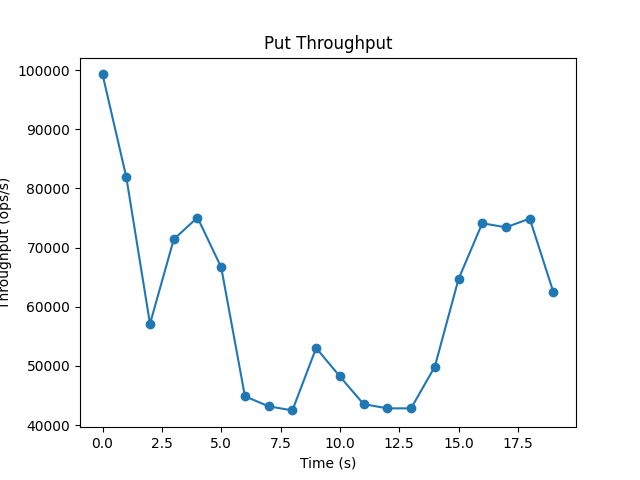
\includegraphics[width=0.5\textwidth]{../imgs/put_plot_test/put_plot_8KB.png}
    \caption{put_throughput}\label{fig:put_throughput}
\end{figure}
可以发现,大趋势是put的吞吐量随时间增加而下降,但是在以秒计数的时间间隔之中,数值抖动明显。原因为:初始时数据较少,合并开销小,吞吐量非常高;\\
而随着时间的增加,合并可能涉及的层数和SSTable个数也越来越多,合并的平均耗时增加。而抖动的原因是,新建一层的大合并(或者任意层数为n)的合并\\
出现所需要的新增键值对个数随指数增长,在一秒的时间间隔内,已经无法保证合并的均匀性,故出现了抖动。



\subsubsection{Bloom Filter 大小配置的影响}

Bloom Filter 大小的影响:Bloom Filter 过大会使得一个 SSTable 中索引数据较少,进而导致 SSTable 合并操作频繁;Bloom Filter 过小又会导致其 false positive 的几率过大,辅助查找的效果不好。\\
你可以尝试不同大小的 Bloom Filter 并保持 SSTable 大小不变,比较系统Get、Put操作性能的差异并思考原因。\\
在我的实验之中,Bloom Filter不同大小带来的效果不太明显,在不同大小Bloom Filter上运行20秒PUT,value_size取100,吞吐量随\\
时间变化的测试结果如下图。

\begin{figure}[h!]
    \centering
    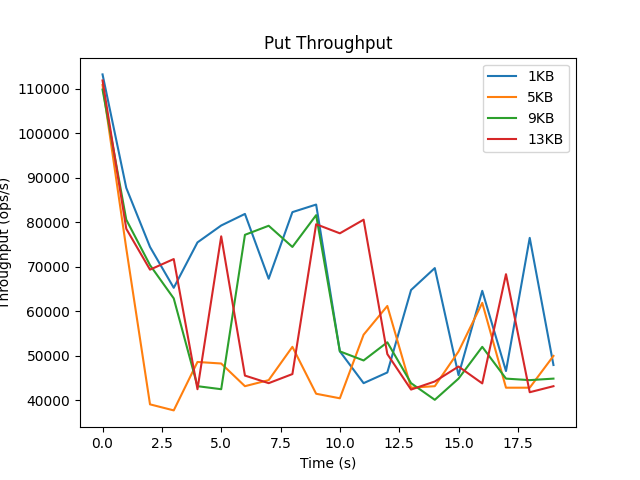
\includegraphics[width=0.5\textwidth]{../imgs/put_plot_test/comparison.png}
    \caption{comparison}\label{fig:comparison}
\end{figure}
可以看到,曲线之间区别较小,原因在于在本次实验之中,性能决定点为vLog的写入部分,而BloomFilter大小的间接影响虽然不小,但相较vLog写入并不是最关键的。



\section{结论}
对 Project 的整体总结,包括对实验结果的评价。
在这个Project之中,我实现了一个具备较高鲁棒性和可用性的LSM键值存储系统,同时通过多种方法实现了较为完备的正确性和性能分析,性能表现符合预期,让我对这个project和对应的LSM树具备了更深刻的理解。

\section{致谢}
(此部分很重要)
在本论文的研究和撰写过程中,我得到了许多人的帮助和支持,在此我要对他们表示最深切的感谢。

首先,我要感谢2022级软件工程专业的同学们,他们在我的学习和研究中提供了很多帮助和建议。特别是廖承凡同学,他在文档的理解交流过程中给予了我巨大的帮助。

其次,我要感谢张迟学长的mini-lsm项目https://github.com/skyzh/mini-lsm ,他对lsm的深入理解和剖析让我对如何改进这个项目有了许多新的想法。我还要感谢google的gtest项目https://github.com/google/googletest ,在这个框架的支持下,项目的测试和维护变得轻松不少。

感谢知乎的文章https://zhuanlan.zhihu.com/p/415799237 ,让我对LSM树的实现有了更加清晰的认识;感谢GeeksforGeeks的一系列算法博客,让我对布隆过滤器和跳表都有了完整和清晰的认识;感谢Effective modern cpp、cppcon和cppreference,在这些书籍、视频和网站的帮助下,我了解了诸多项目中需要用的现代c++的语法知识。

\section{其他和建议}
这部分不做强制要求,你可以列出 LSM-KV Project中遇到的种种困难、挑战、bug、以及吐槽。

困难与挑战:主要在于对modern cpp语法的不了解和c++文件操作带来的debug困难,这个project是一次很好的TDD(测试驱动开发)的实践,在不断地写单元测试、跑单元测试和回归测试的过程之中,我对每个子模块和整体的项目的正确性和架构如何解耦产生了许多新的认知。如何对持久化操作测试是有挑战的。

bug: 印象最深的有两个:一个是传了vector的引用进一个函数,但在函数内部同时修改vector和使用vector的迭代器/引用——造成了重定位带来的迭代器失效问题;还有一个是在布隆过滤器的函数的实现里面捕获了一个悬垂指针。

吐槽:最后我的单测写得比代码都多了,感觉可以再给多一些单测,这是其一;助教的测试用例用"sssssss..."根本无法debug,这是其二;这个试验报告要测试的东西也太多了,我python脚本和c++测试文件又写了四五百行.......,这是其三。


% \bibliography{references.bib}


\end{document}

